\documentclass{sig-alternate}
\usepackage[numbers, sort, compress]{natbib}
\usepackage{graphics}
\usepackage{graphicx}
\usepackage{epstopdf}
\usepackage{color}
\usepackage{hyperref}
\usepackage{pdfsync}
\usepackage{mdwlist}


\begin{document}

\conferenceinfo{} {}
\CopyrightYear{2011}
\crdata{}
%\clubpenalty=10000
%\widowpenalty = 10000


\title{A Practical Comparison of NGS Short Read Aligners : Data-Intensive Distributed Computing Perspective}

\numberofauthors{6}
\author{
\alignauthor Joohyun Kim\titlenote{Author for correspondence, e-mail : jhkim@cct.lsu.edu}\\
       \affaddr{Center for Computation and Technology}\\
       \affaddr{Louisiana State University}\\
       \affaddr{216 Johnston}\\
       \affaddr{Baton Rouge, LA} \\
  %     \email{jhkim@cct.lsu.edu}
\alignauthor Sharath Maddineni\\
       \affaddr{Center for Computation and Technology}\\
       \affaddr{Louisiana State University}\\
       \affaddr{216 Johnston}\\
       \affaddr{Baton Rouge, LA}
   %    \email{smaddineni@cct.lsu.edu}
\alignauthor Mark Santcroos\\
       \affaddr{Center for Computation and Technology}\\
       \affaddr{Louisiana State University}\\
       \affaddr{216 Johnston}\\
       \affaddr{Baton Rouge, LA}
  %     \email{}
       \and
\alignauthor Ole Weidner\\
       \affaddr{Center for Computation and Technology}\\
       \affaddr{Louisiana State University}\\
       \affaddr{216 Johnston}\\
       \affaddr{Baton Rouge, LA}
%       \email{oweinder@cct.lsu.edu}
\alignauthor Shantenu Jha\titlenote{Author for correspondence, e-mail : sjha@cct.lsu.edu}\\
      \affaddr{Center for Computation and Technology}\\
     \affaddr{Louisiana State University}\\
      \affaddr{214 Johnston}\\
      \affaddr{Baton Rouge, LA}
%     \email{sjha@cct.lsu.edu}
}

\maketitle



\begin{abstract}
We present the comparison of short read aligners for Next-Generation Sequencing (NGS) data.  The main goal of the comparison is to understand the possible utilization of each aligner with Data-Intensive Distributed Computing (DIDC).  To this end, first, we characterized computational requirements and implementation strategies, and then  outputs obtained with two classes of genomes, a microbe, Bukerholderia Glumae and human (hg18), which together allowed us to find favorable usage modes of aligners with scalable distributed resources.  

With several widely used, publicly accessible aligners selected for this comparison, this work provides useful information on i) how the strategy with DIDC could advance NGS analytics in particular by keeping the total time-to-completion of alignment desirably low without compromising ideal sensitivity of an individual aligner and ii) how a desirable workflow for NGS analytics and downstream analyses with emerging scalable distributed computing environments such as HPC grids and Clouds would be constructed by considering computational characteristics and     
algorithmic implementation decided by developers.  
  
\end{abstract}

\newif\ifdraft
%\drafttrue                                                                                        \
\ifdraft
% \newcommand{\reviewer}[1]{ {\textcolor{blue}    { ***Reviewer:     #1 }}}
 \newcommand{\jkimnote}[1]{{\textcolor{green}   { ***Joohyun:   #1 }}}
 \newcommand{\jhanote}[1]{  {\textcolor{red}     { ***SJ: #1 }}}
  \newcommand{\smnote}[1]{  {\textcolor{red}     { ***Sharath: #1 }}}
 \newcommand{\todo}[1]{  {\textcolor{red}     { ***TODO: #1 }}}
 \newcommand{\fix}[1]{  {\textcolor{red}     { ***FIX: #1 }}}
 \newcommand{\reviewer}[1]{}
\else
 \newcommand{\reviewer}[1]{}
 \newcommand{\jkimnote}[1]{}
 \newcommand{\smnote}[1]{}
 \newcommand{\jhanote}[1]{}
 \newcommand{\todo}[1]{  {\textcolor{red}     { ***TODO: #1 }}}
 \newcommand{\fix}[1]{}                                                                              
 \fi



\category{D.1.3}{Software}{Concurrent Programming}{ Distributed programming/parallel programming} 
\category{J.3}{Computer Applications}{Bioinformatics}

  
\section*{General Terms}{Design,Measurement,Theory}

 \keywords{Short-read Aligner, Distributed Computing, Simple API for Grid
  Applications (SAGA), Pilot-Job abstraction, Data-intensive Computing}

\section{INTRODUCTION}

%\begin{figure}
% \centering
%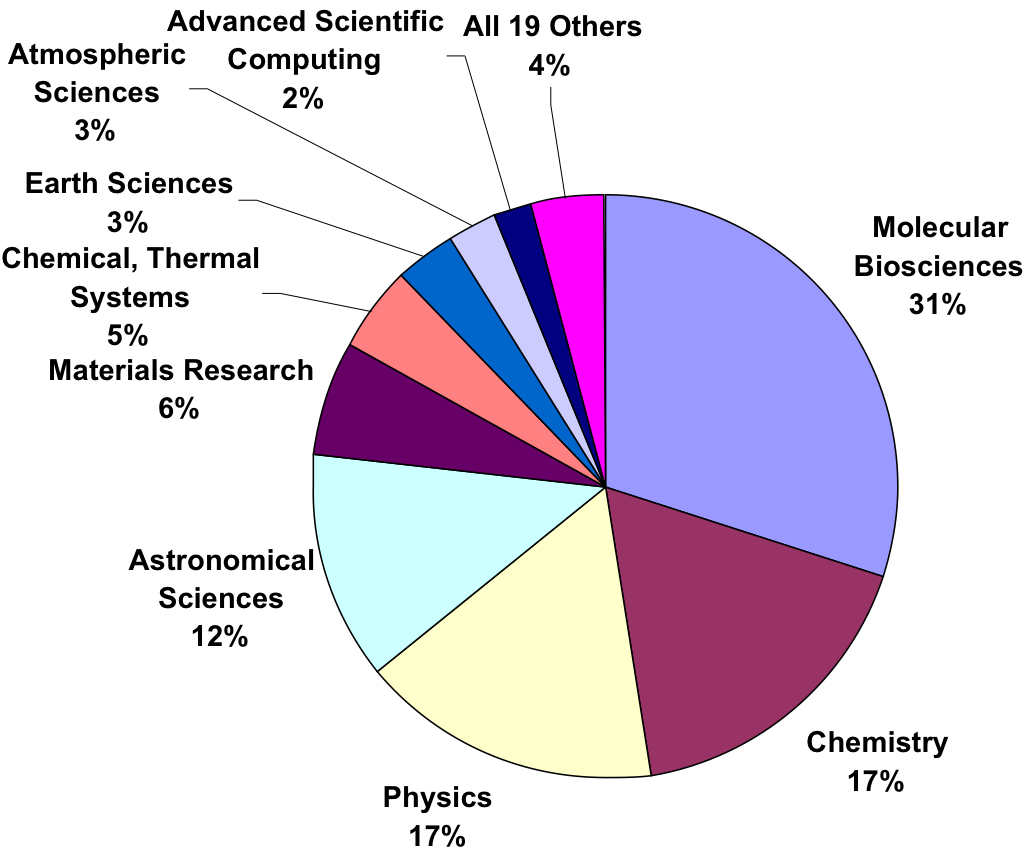
\includegraphics[scale=0.40]{figures/teragrid-discipline07}
%\caption{\small 2007 Usage statistics for the TeraGrid.  (Reference
%  \url{http://www.teragridforum.org/mediawiki/images/9/90/II_WorkShop_G-HPC_Nework_2009-Towns.pdf})}
%  \label{tg2007}
%\end{figure}

The alignment of massively generated short reads from High-throughput Sequencing techniques such as Next-Generation Sequencing platforms is the first step, along with de novo assembly, of biological discovery aiming genome structure variation, transcriptome analysis, and genome-wide DNA-protein interaction profiling.  

In recent years, new programs were introduced in the NGS community many of which improved sensitivity by employing better algorithms for locating candidate match locations, and the final local alignment allowing gapped match.  Still, computing power is one of primary concerns of developers due to large memory requirement as well as disk space for large eukaryote genomes, resulting in a conventional consensus that the balance between sensitivity and computational requirement.  However, as we recently addressed, distributed computing could remove the major obstacle associated with computational requirement by providing a runtime environment for a aligner, and therefore encourages the next generation of alignment programs only focusing on the sensitivity.    

Another aspect, which does not draw serious attention from the community, is the use of multiple programs.  Carrying out multiple aligners and utilize all produced information for downstream analyses is the strategy that most of researchers with NGS technologies concede as an ideal one, but in a practical setting, it is a non-trivial task.      

Motivated by such observations, we explore essential information for our new approach for NGS mapping, providing the Data-Intensive Distributed Computing that executes multiple mappers regardless of their computing requirement with scalable computing environment such as HPC grids, Clouds, and HTC grids.


\begin{table}
 \small
\begin{tabular}{|c|c|c|c|c|} 
  \hline  
& BFAST  & BWA & Novo- & SHRiMP2  \\  
&  &  & align & \\ \hline \hline
\textbf{INDEXING}  & & & &  \\
 Algorithm & HT & BWT & HT & HT \\
 Target & Ref & Ref & Ref & Ref \\ \hline
\textbf{SEARCH} & & & & \\
Space Seed & Yes &   &  Yes & \\ \hline
\textbf{ALIGNMENTt} &  & & & \\
Gapped & Yes & Yes & Yes & Yes \\ 
Algorithm & SW & SW & NW & \\ 
Paired-End &  &  &  & \\ \hline
\textbf{MISC}  &  &  &  & \\
Color Space Support  & Yes & Yes & Yes & Yes  \\
Sam Output & Yes & Yes & Yes &   \\ \hline
\textbf{FINE-GRAIN} &  &  &  & \\ 
 \textbf{PARALLELISM} & & & & \\
Multi-Threading & Yes & Yes & Yes & Yes\\ 
MPI & & & Yes &\\
OpenMP &  & &  & Yes \\  \hline
\textbf{COARSE-GRAIN}  & & & &\\ 
\textbf{PARALLELISM} & & & & \\\
& & & &  \\ \hline
\end{tabular} 

\begin{tabular}{|c|c|c|c|c|} 
  \hline  
& SOAP2  & Stampy & Bowtie & MAQ  \\  \hline \hline
\textbf{INDEXING}  & & & &  \\
 Algorithm & BWT &  & BWT & HT \\
 Target &  &  & & Reads \\ \hline
\textbf{SEARCH} & & & & \\
Space Seed &  &   &   & \\ \hline
\textbf{ALIGNMENT} &  & & & \\
Gapped &  & & No &  \\ 
Algorithm & &  &  & \\ 
Paired-End &  &  &  & \\ \hline
\textbf{Misc}  &  &  &  & \\ 
Color Space Support  & No &  &  &   \\
Sam Output & &  &   & \\  \hline
\textbf{FINE-GRAIN} &  &  &  & \\ 
 \textbf{PARALLELISM} & & & & \\
Multi-Threading &  &  &  & \\ 
MPI & & & Yes &\\
OpenMP &  & &  & Yes \\  \hline
\textbf{COARSE-GRAIN}  & & & &\\ 
\textbf{PARALLELISM} & & & & \\\
& & & &  \\ \hline
\end{tabular} 



\caption{Overall comparison of the mapping tools or aligners surveyed in this work. HT : Hash Table, BWT : Burrow Wheeler Transform, SW : Smith-Waterman, NW : .  MPI : Message Passing Interface}
 \label{tbl:comp-aligner} 
\end{table}


\section{Algorithmic Characteristics}






\textit{Reference genome indexing}



\textit{Alignment candidate finding}


\textit{Local alignment}



\section{Computational Requirement}
\textit{Fine-grain parallelism support}



\textit{Reference index management}


\textit{Task level concurrency support}






\begin{table}

\begin{tabular}{|c|c|c|c|}  \hline
  & Memory & Disk-space & Supporting     \\ 
  &  &    & Parallelism \\ \hline 
\textbf{BFAST} &  &  & \\
index  & 16 GB & 130 GB & \\ 
match & &  &  \\ 
localalignalign & & &  \\
postprocess & &  &  \\ \hline
\textbf{BWA} & & & \\
index &  & & \\
aln &  &  & \\
sampe &  &  & \\  \hline


\end{tabular} 
\caption{Comparison of computational requirement for memory and disk space with a standard condition and supported parallelism.  Here, a standard condition represents computation without parallelism, i.e. using a single processor with a single file for a reference genome (fasta) and a short read data file (fastq).   In general, tools surveyed in this work are composed of multiple steps. The requirement is analyzed for each step. The NGS data used are the human exome data sets obtained from the SOLiD platform and a microbial genome data from Illumina GA II.}
 \label{comp-req-bfast} 
\end{table}




\section{Dat-intensive Computing as a Distributed Application}


\section{Conclusions}



\section{Acknowledgments}
We are grateful to Andre Luckow for his work for SAGA-BigJob development.  Computing resources used for this
work were made possible via NSF TRAC award TG-MCB090174 and LONI
resources.  This document was developed with support from the National
Science Foundation (NSF) under Grant No.  0910812 to Indiana
University for ``FutureGrid: An Experimental, High-Performance Grid
Test-bed.'' The project described was partially supported by Grant
Number P20RR016456 from the NIH National Center For Research
Resources. SJ would like to thank Dave Hart (SDSC) and Dan Katz
(Chicago) for helpful discussions.

\bibliographystyle{abbrv}
\bibliography{}
\end{document}



% \textit{Achieving IDEAS : Interoperability, Distributed
%   scaled-out, Extensibility, Adaptivity, and Simplicity}

%\smnote{ 1) Lets say we have "n" read files and with DARE it takes
%  around time "t" time for matching step if we run it serially it
%  would take n*t time. It probably exceeds wall time limit. Therefore
%  speed up in match step depends how many number of read files we
%  generate and process concurrently.  2) Yes we were able to process
%  the complete run with entire Human Genome on QB and Ranger
%  separately. (**I am currently working this to utilizing QB and
%  Ranger together.)  4) it should clearly provide the advantage with
%  multiple resources. If we want to use the cloud resources from India
%  to complete Human Genome run it is not practically possible because
%  of the current limited disk size access provided by the FG
%  Eucalyptus resources. Because whole human genome index files are of
%  size 129 GB for Bfast matching step as opposed to HG 18 Chromosome
%  21 with size of 2 GB index files. On the other hand it also requires
%  the temporary files disk space.  Thus it is important to utilize
%  large capacity resources like QB and Ranger divide the work load
%  across machines.}  
  
%   Here, we present how the objectives of IDEAS\cite{ideas} are
% accomplished with the DARE gateway examples. 
